% Options for packages loaded elsewhere
\PassOptionsToPackage{unicode}{hyperref}
\PassOptionsToPackage{hyphens}{url}
\PassOptionsToPackage{dvipsnames,svgnames,x11names}{xcolor}
%
\documentclass[
  letterpaper,
  abstract]{scrartcl}

\usepackage{amsmath,amssymb}
\usepackage{iftex}
\ifPDFTeX
  \usepackage[T1]{fontenc}
  \usepackage[utf8]{inputenc}
  \usepackage{textcomp} % provide euro and other symbols
\else % if luatex or xetex
  \usepackage{unicode-math}
  \defaultfontfeatures{Scale=MatchLowercase}
  \defaultfontfeatures[\rmfamily]{Ligatures=TeX,Scale=1}
\fi
\usepackage{lmodern}
\ifPDFTeX\else  
    % xetex/luatex font selection
\fi
% Use upquote if available, for straight quotes in verbatim environments
\IfFileExists{upquote.sty}{\usepackage{upquote}}{}
\IfFileExists{microtype.sty}{% use microtype if available
  \usepackage[]{microtype}
  \UseMicrotypeSet[protrusion]{basicmath} % disable protrusion for tt fonts
}{}
\makeatletter
\@ifundefined{KOMAClassName}{% if non-KOMA class
  \IfFileExists{parskip.sty}{%
    \usepackage{parskip}
  }{% else
    \setlength{\parindent}{0pt}
    \setlength{\parskip}{6pt plus 2pt minus 1pt}}
}{% if KOMA class
  \KOMAoptions{parskip=half}}
\makeatother
\usepackage{xcolor}
\usepackage[margin=1.1in,letterpaper]{geometry}
\setlength{\emergencystretch}{3em} % prevent overfull lines
\setcounter{secnumdepth}{5}
% Make \paragraph and \subparagraph free-standing
\ifx\paragraph\undefined\else
  \let\oldparagraph\paragraph
  \renewcommand{\paragraph}[1]{\oldparagraph{#1}\mbox{}}
\fi
\ifx\subparagraph\undefined\else
  \let\oldsubparagraph\subparagraph
  \renewcommand{\subparagraph}[1]{\oldsubparagraph{#1}\mbox{}}
\fi


\providecommand{\tightlist}{%
  \setlength{\itemsep}{0pt}\setlength{\parskip}{0pt}}\usepackage{longtable,booktabs,array}
\usepackage{calc} % for calculating minipage widths
% Correct order of tables after \paragraph or \subparagraph
\usepackage{etoolbox}
\makeatletter
\patchcmd\longtable{\par}{\if@noskipsec\mbox{}\fi\par}{}{}
\makeatother
% Allow footnotes in longtable head/foot
\IfFileExists{footnotehyper.sty}{\usepackage{footnotehyper}}{\usepackage{footnote}}
\makesavenoteenv{longtable}
\usepackage{graphicx}
\makeatletter
\def\maxwidth{\ifdim\Gin@nat@width>\linewidth\linewidth\else\Gin@nat@width\fi}
\def\maxheight{\ifdim\Gin@nat@height>\textheight\textheight\else\Gin@nat@height\fi}
\makeatother
% Scale images if necessary, so that they will not overflow the page
% margins by default, and it is still possible to overwrite the defaults
% using explicit options in \includegraphics[width, height, ...]{}
\setkeys{Gin}{width=\maxwidth,height=\maxheight,keepaspectratio}
% Set default figure placement to htbp
\makeatletter
\def\fps@figure{htbp}
\makeatother

\KOMAoption{captions}{tableheading}
\makeatletter
\@ifpackageloaded{caption}{}{\usepackage{caption}}
\AtBeginDocument{%
\ifdefined\contentsname
  \renewcommand*\contentsname{Table of contents}
\else
  \newcommand\contentsname{Table of contents}
\fi
\ifdefined\listfigurename
  \renewcommand*\listfigurename{List of Figures}
\else
  \newcommand\listfigurename{List of Figures}
\fi
\ifdefined\listtablename
  \renewcommand*\listtablename{List of Tables}
\else
  \newcommand\listtablename{List of Tables}
\fi
\ifdefined\figurename
  \renewcommand*\figurename{Figure}
\else
  \newcommand\figurename{Figure}
\fi
\ifdefined\tablename
  \renewcommand*\tablename{Table}
\else
  \newcommand\tablename{Table}
\fi
}
\@ifpackageloaded{float}{}{\usepackage{float}}
\floatstyle{ruled}
\@ifundefined{c@chapter}{\newfloat{codelisting}{h}{lop}}{\newfloat{codelisting}{h}{lop}[chapter]}
\floatname{codelisting}{Listing}
\newcommand*\listoflistings{\listof{codelisting}{List of Listings}}
\makeatother
\makeatletter
\makeatother
\makeatletter
\@ifpackageloaded{caption}{}{\usepackage{caption}}
\@ifpackageloaded{subcaption}{}{\usepackage{subcaption}}
\makeatother
\ifLuaTeX
  \usepackage{selnolig}  % disable illegal ligatures
\fi
\usepackage[sorting=none, style=numeric-comp]{biblatex}
\addbibresource{../library.bib}
\usepackage{bookmark}
\usepackage{xcolor}
\definecolor{myorange}{RGB}{240, 96, 0}
\newcommand{\mt}[1]{{\textcolor{myorange} {({\tiny MT:} #1)}}}
\newcommand\numberthis{\addtocounter{equation}{1}\tag{\theequation}}

\IfFileExists{xurl.sty}{\usepackage{xurl}}{} % add URL line breaks if available
\urlstyle{same} % disable monospaced font for URLs
\hypersetup{
  pdftitle={Predicting the effect of candidate interventions for mitigating disease spread in asymmetric mixing metapopulations},
  colorlinks=true,
  linkcolor={blue},
  filecolor={Maroon},
  citecolor={Blue},
  urlcolor={Blue},
  pdfcreator={LaTeX via pandoc}}

\title{Predicting the effect of candidate interventions for mitigating
disease spread in asymmetric mixing metapopulations}
\author{Matthew Adam Turner}
\date{}

\begin{document}
\maketitle
\begin{abstract}
\noindent hello
\end{abstract}

\renewcommand*\contentsname{Table of contents}
{
\hypersetup{linkcolor=}
\setcounter{tocdepth}{3}
\tableofcontents
}
\section{Introduction}\label{introduction}

To equitably prepare for pandemics in our uncertain world we need to
\autocite{Rodo2021,Adashi2022}. The global COVID-19 pandemic highlighted
the current lack of outcome equality, where a country's inequality
(measured by the Gini index) predicted higher burden of COVID-19
infections \autocite{Su2022}. Here we contribute to this program of more
equitable pandemic preparedness by developing a compartmental
behavioral-epidemiological metapopulation model of COVID-19 transmission
between a Brazilian city, Dourados, in Mato Grosso do Sul, and the
neighboring Dourados Indigenous Reserve \autocite{DeOliveira2023}.
COVID-19 burden was felt disproportionately by Indigenous peoples in
Brazil \autocite{Simionatto2020}, but may have been worse in the
Dourados Reserve due to its immediate proximity to the Dourados. Nearly
all residents of the reserve live in domiciles in one of two villages in
the Reserve, Jaguapiru and Bororó. Jaguapiru is closer overall to the
city of Dourados, sharing a much longer border with the city limits than
Bororó (Figure 1). Indigenous peoples on the reserve are predominantly
one of two ethnicities, Guarani and Terena. Anecdotally, Terena are
known for being better educated with somewhat more robust physicality
and, perhaps, better resistance to disease. They may travel to the city
more frequently for trade and other purposes.

De Oliveira and co-authors hypothesized that COVID-19 variant diffusion
from Dourados City into the Dourados Reserve is driven by young
Indigenous men traveling between the reserve and the city of Dourados
for economic reasons. This is a reasonable hypothesis given available
data.

\begin{figure}[H]

{\centering 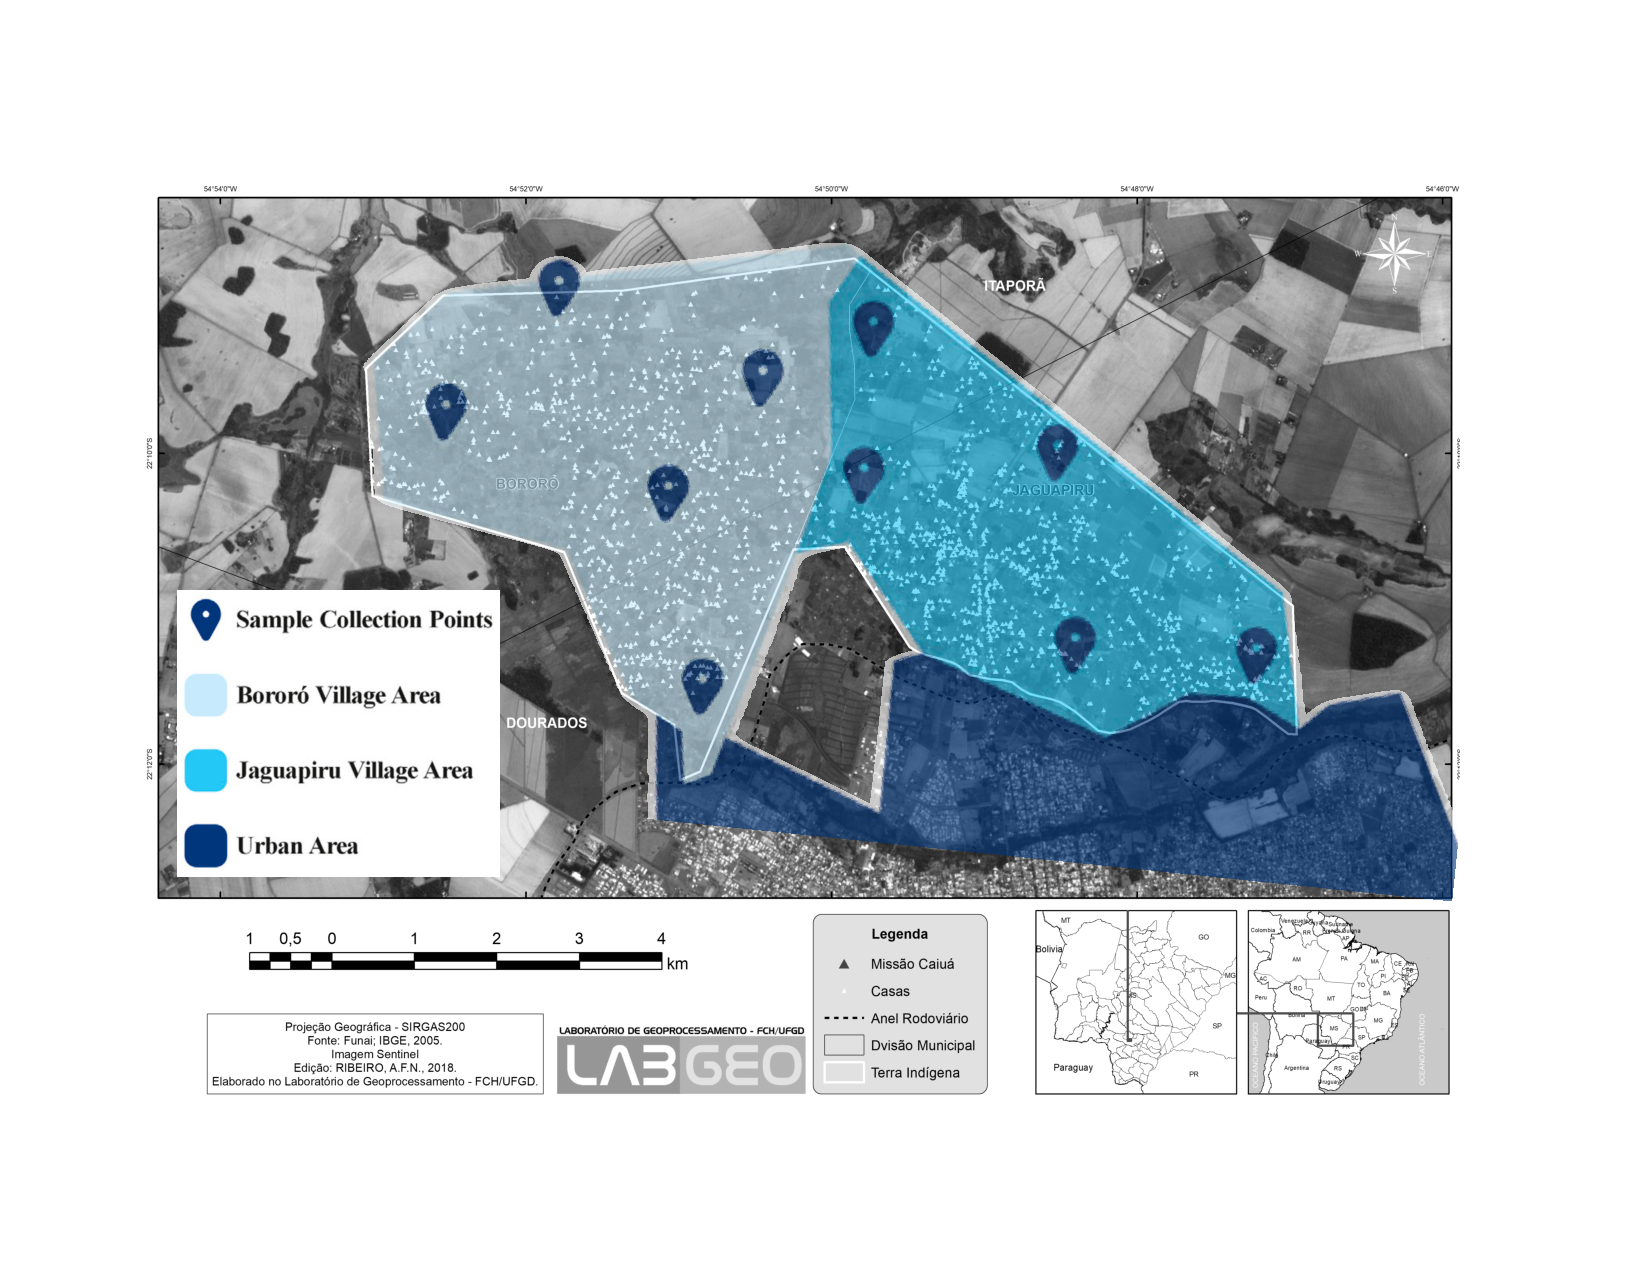
\includegraphics[width=0.8\textwidth,height=\textheight]{Figures/ReserveMap.pdf}

}

\caption{Map of Dourados Indigenous Reserve villages (Bororó in light
blue, Jaguapiru in cyan) and the city of Dourados (dark blue). Note
Jaguapiru shares a much longer boundary with the reserve than Dourados,
which facilitates mobility in and out of the reserve for both Reserve
and city residents. Maps combined from Schnaufer et al.~(2023) and
Cavalcante (2019)}

\end{figure}%%
\begin{figure}[H]

{\centering \includegraphics[width=0.8\textwidth,height=\textheight]{Figures/Time Series.pdf}

}

\caption{Time series of COVID-19 spread through the Dourados Indigenous
Reserve, with significant events highlighted. The first B.1.1 variant
cases were introduced by the Guarani ethnicity (1), followed about one
month later by a rapid rise in cases in Jaguapiru among the Terena
ethnicity(2); several months later a rapid rise in Bororó was caused by
a rapid rise among Guarani (3). Zeta was introduced at the end of 2020
(4), with a rapid rise around the holiday season especially in Jaguapiru
among Guarani (5); later in February cases rose in Bororó among the
Terena (6).}

\end{figure}%

Despite some evidence to support the hypothesis that young male
Indigenous mobility can explain transmission into the reserve, there are
many complicating factors that make it difficult to evaluate this
hypothesis directly without adding some additional qualifications. There
may be other social factors that may be necessary for the time series
observations of De Oliveira and co-authors. Furthermore, there may be
less significant factors driving transmission in this model that may be
of greater importance in future outbreaks of different diseases than
SARS-CoV-2 in the reserve. Therefore, here we expand the scope of the
hypothesis to include hypotheses about how social groups, namely village
residency and Indigenous ethnic group, affect transmission in the
reserve and explain observed outbreaks of variants B.1.1 and Zeta in the
Reserve. To evaluate the hypotheses, presented in the next paragraph, we
develop a mechanistic model of epidemiological transmission with
asymmetric social mixing that evaluates how best to model group
structure in the Reserve. In turn, this model is used to evaluate
potential economic interventions that target aid to different groups to
reduce infections in the reserve.

\begin{itemize}
\item
  De Oliveira and colleagues tracked the spread of different SARS-CoV-2
  variants by village and by variant.
\item
  The goal of our model is two-fold. First, to identify parameters that
  could re-create the time series plots in Figure 1.
\item
  Second, we aim to use a parameterized model to understand how
  different intervention strategies could reduce infections among
  Reserve residents. For example, perhaps since Terena are suspected to
  travel to the
\item
  While we know a lot about transmission in the reserve, and the work of
  de Oliveira and colleagues advanced our understanding of transmission
  in the Reserve, we do not have reliable estimates of exactly how many
  cases there were per ethnicity and village. We also have only
  word-of-mouth information about the frequency of travel to the city
  for each ethnicity and location. Our model motivates the need for a
  more thorough understanding of behavior and epidemiological parameters
  in the Dourados Indigenous Reserve, and points the way towards future
  research in other Indigenous communities, and more complex situations.
  Here we only consider Indigenous mobility, but many people from the
  city travel to the reserve for commerce as well.
\end{itemize}

\section{Model}\label{model}

\begin{figure}[H]

{\centering \includegraphics{Figures/ModelSketch.pdf}

}

\caption{\mt{UPDATE THIS CAPTION AND THE FIGURE TO MATCH EQUATIONS. ADD PARAMETERS TABLE.}
  We can model the relevant groups for mixing as either village
residence or ethnicity. Transmission, mixing, and mobility parameters
would be set accordingly. The \(C_g\) parameters would be reduced if
economic aid were allocated to keep group \(g\) on the Reserve during
outbreaks.}

\end{figure}%

\subsection{Equations}\label{equations}

\begin{align*}
  \frac{dS_g}{dt} &= -\left(\tau c_{gg'} I_g + c_{g'g}I_{g'} + \gamma_g \right)S_g + r R_g   \\
  \frac{dI_g}{dt} &= \left(\tau c_{gg'} I_g + c_{g'g}I_{g'} + \gamma_g \right)S_g - \rho I_g \\
  \frac{dR_g}{dt} &= \rho I_g - r R_g
    \numberthis \label{eq:DiseaseContagion}
\end{align*}
\noindent

\section{Analysis (Sketch)}\label{analysis-sketch}

\begin{figure}[H]

{\centering \includegraphics[width=0.95\textwidth,height=\textheight]{Figures/ResultsSketch_ReductionByGroup.pdf}

}

\caption{Global reduction in travel to and from the city could have
differential effects on reduction in incidence for different groups.}

\end{figure}%


\begin{figure}[H]

{\centering \includegraphics[width=0.95\textwidth,height=\textheight]{Figures/ResultsSketch_ByStrategy.pdf}

}

\caption{We hypothesize that overall reduction in disease incidence ($\Delta I$, y-axis)  depends on 
strategy to distribute the total aid to reduce travel between Dourados Reserve and city ($\gamma$, x-axis).}

\end{figure}%

\section{Discussion}\label{discussion}


\begin{itemize}
  \item 
    Application to other problematic diseases in the Reserve, e.g., TB, STDs,\ldots 
  \item
    The data is not necessarily representative and we had to use educated guesses
    for mixing parameters.
\end{itemize}


\printbibliography[title=References]


\end{document}
